\newpage
\section{GPIO}
    \subsection{GPIO-Erklärung}
    Wie man bei der Abbildung \ref{caption:System-Architektur} sehen kann, sind die GPIOs am BUS AHB2 verbunden. 
    Da das verwendete Paket nur GPIO A verwendet müssen dementsprechend die GPIO-A Register richtig konfiguriert werden\\
    Das Register um die GPIOs als output einzustellen ist \textbf{GPIOA\_MODER im Addressraum 0x4800 0000 (des AHB2 Buses) mit dem Address offset: 0x00}\\
    Um Pins für die UART verwenden zu können müssen diese Pins noch als $"$alternate functions$"$ konfiguriert werden im Register \textbf{GPIOA\_AFRH mit Address offset: 0x24}.
    Welche Pin Nummer man Programmieren muss, sieht man in der Abbildung \ref{caption:GPIO-UART-PIN-Table}, man benötigt PA9 (Pin:17) und PA10 (Pin:18), da diese als alternate function
    die USART\_1 TX und RX hinterlegt haben. Wie das alternate function Register konfiguriert werden muss sieht man in den Abbildungen \ref{caption:GPIO-AF} 
    und \ref{caption:GPIO-AF-Register}\\\\
    Weiterhin müssen noch zwei GPIO Pins Für die DE und RE Pins des MAX485 als output konfiguriert werden. Ich verwend PA7 und PA8.\\
    Ebenfalls wird ein GPIO Pin als analog konfiguriert um diesen als ADC Eingang zu verwenden. 
    

    \begin{figure}[!htb]
        \centering
        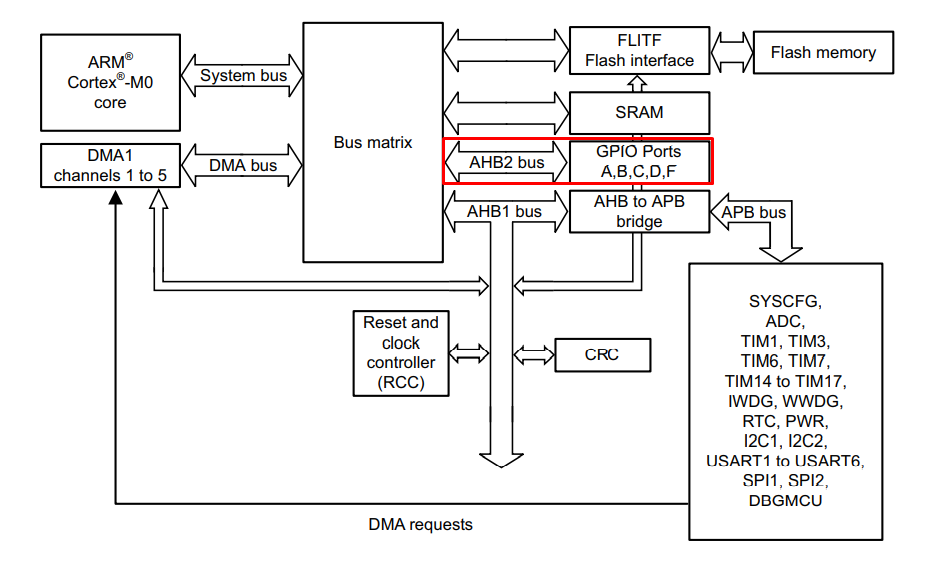
\includegraphics[width=\linewidth]{System-Architektur.png}
        \caption{System-Architektur}
        \label{caption:System-Architektur}
    \end{figure}

\newpage
    \begin{figure}[!htb]
        \centering
        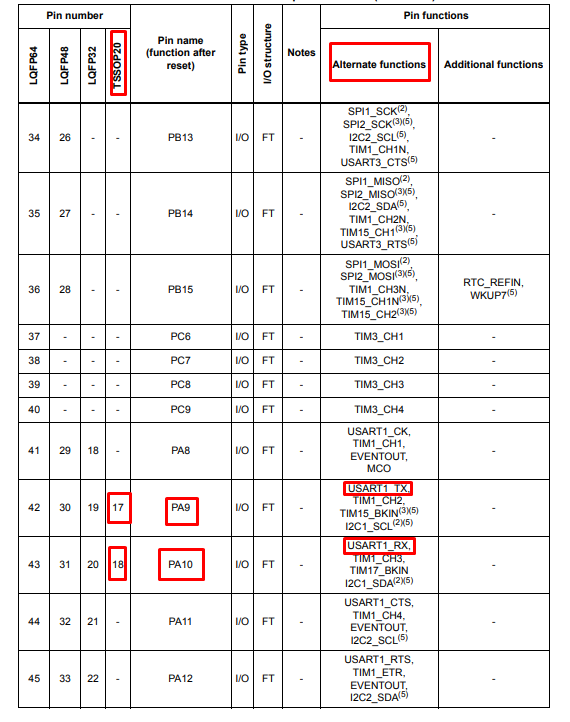
\includegraphics[scale=0.90]{GPIO-UART-PIN-Table.png}
        \caption{GPIO-UART-PIN-Table}
        \label{caption:GPIO-UART-PIN-Table}
    \end{figure}

\newpage
    \begin{figure}[!htb]
        \centering
        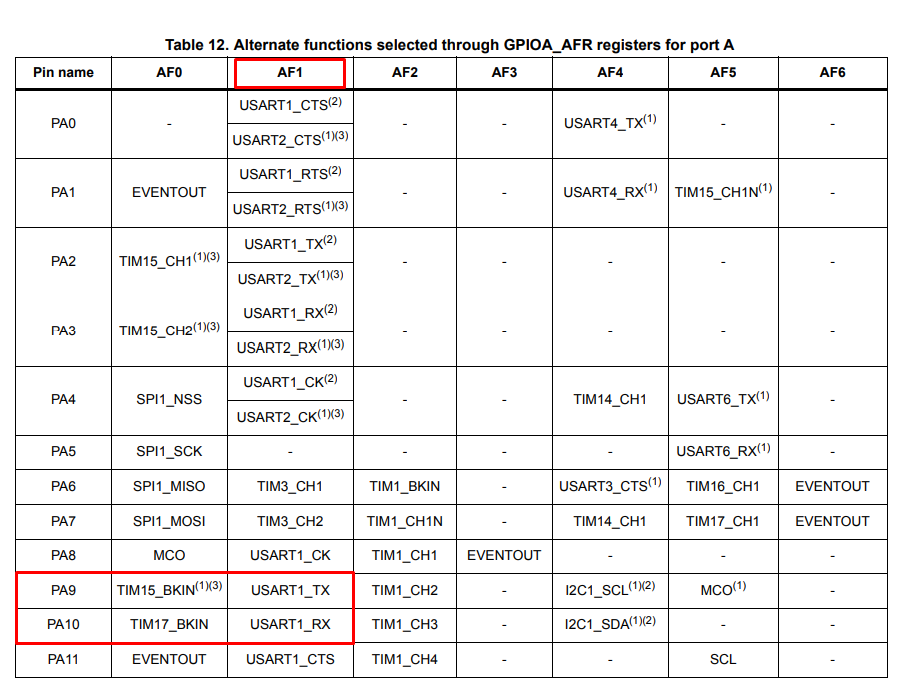
\includegraphics[scale=0.65]{GPIO-AF.png}
        \caption{GPIO-AF}
        \label{caption:GPIO-AF}
    \end{figure}
    
\newpage
    \begin{figure}[!htb]
        \centering
        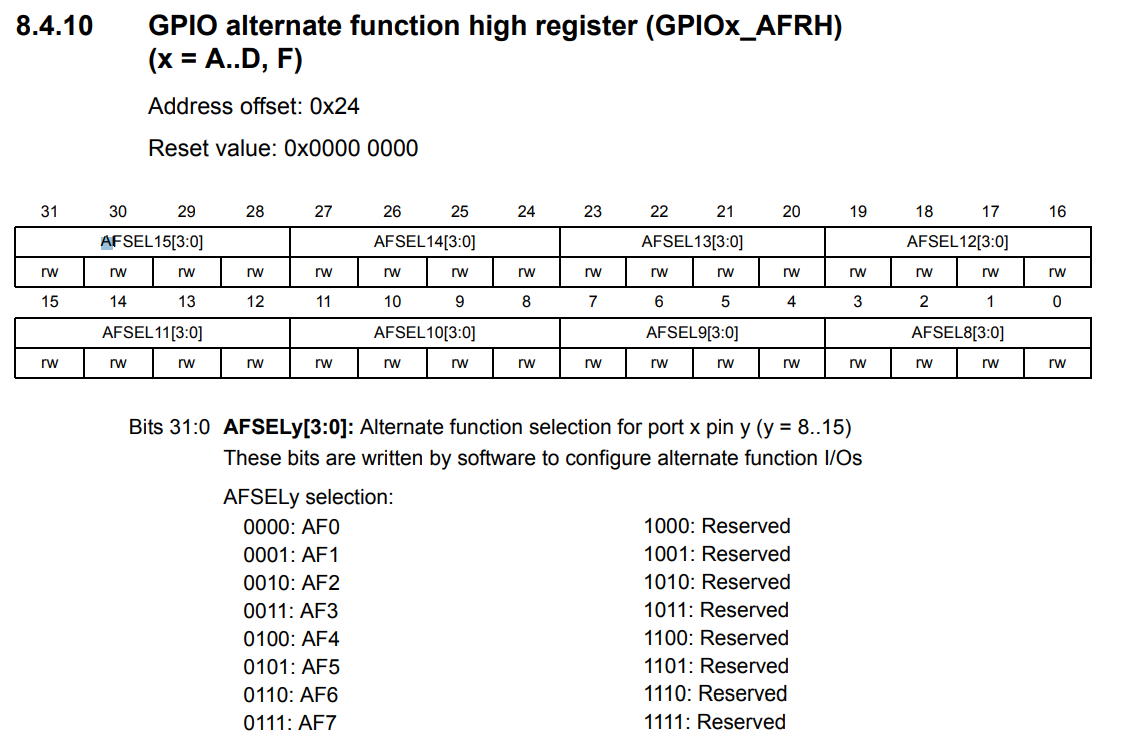
\includegraphics[scale=0.65]{GPIO-Alternate-function.png}
        \caption{GPIO-AF-Register}
        \label{caption:GPIO-AF-Register}
    \end{figure}
        
\newpage
\subsection{GPIO-Code}
    \begin{lstlisting}[language=C, style=CStyle, caption=GPIO-Code, captionpos=b, label=GPIO-Code]
int init_GPIO()
{
    //Set GPIO pins PA9 and PA10 alternate function for USART TX and RX, 
    //set PA7 and PA6 output for DE and RE of MAX485 
    //PA0 ADC_IN0 so set it to analog and then in DAC register set PA0 as ADC_IN0 
    uint32_t reg_content;
    uint32_t* gpioa_moder = GPIOA_MODER;
    uint32_t* gpioa_afrh = GPIOA_AFRH;
    uint32_t* gpioa_odr = GPIOA_ODR;

    reg_content = *gpioa_moder;
    reg_content |= 0x00285003;
    *gpioa_moder = reg_content;

    //Set GPIO PA9 as AF=TX and PA10 as AF = RX
    reg_content = *gpioa_afrh;
    reg_content |= 0x00000110;
    *gpioa_afrh = reg_content;

    //Ensure that output gpios are 0 for MAX, to read all the time
    //and only send, when needing to send
    reg_content = *gpioa_odr;
    reg_content |= 0x00000000;
    *gpioa_odr = reg_content;  
}
    \end{lstlisting}
        
    
    
    
    % \begin{figure}[!htb]
    %     \centering
    %     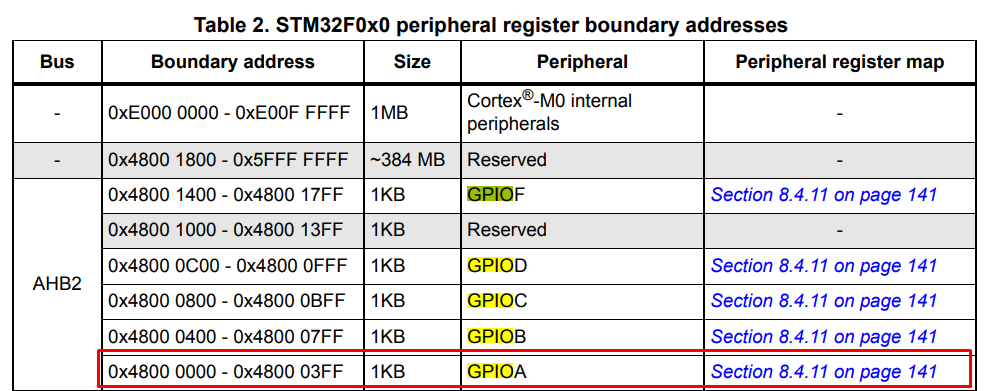
\includegraphics[scale=1]{GPIO-A-Boundary-address.png}
    %     \caption{GPIO-A-Boundary-address}
    %     \label{caption:GPIO-A-Boundary-address}
    % \end{figure}


    % \begin{figure}[!htb]
    %     \centering
    %     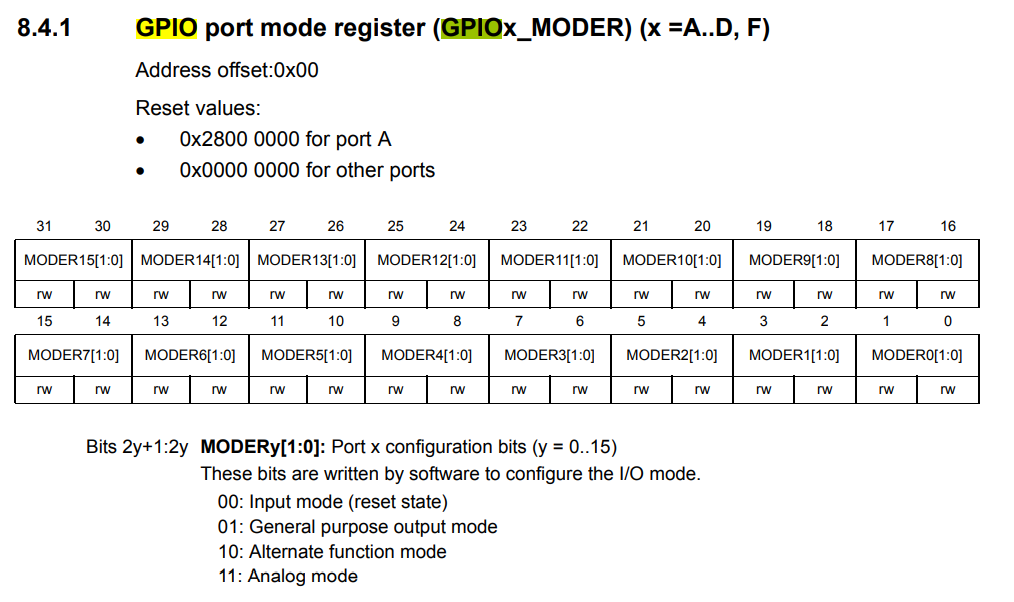
\includegraphics[scale=1]{GPIOx-Register.png}
    %     \caption{GPIOx-Register}
    %     \label{caption:GPIOx-Register}
    % \end{figure}


    
